\documentclass[a4paper,14pt]{extarticle}
\usepackage[utf8]{inputenc}
\usepackage[thinlines]{easytable}
\usepackage{enumitem}
\usepackage{tikz}
\usepackage{geometry}
\usepackage{extsizes}
\usepackage{titling}
\usepackage[document]{ragged2e}
\usepackage{pgfplots}
\usetikzlibrary{datavisualization}
\usetikzlibrary{datavisualization.formats.functions}
\graphicspath{ {./images/} }

\geometry{left=1cm, right=1cm, top=1cm, bottom=2cm}
\title{\vspace{-2cm}\textbf{Algebra 2}}
\author{}
\date{}

\begin{document}
% Title
\maketitle

% Q1
\vspace{-4.5cm}
\begin{enumerate}
\item Graphing Linear Equations 
\begin{enumerate}
\item
\par{Graph the line $y = 2x + 4$ and, hence, solve for $x$ if $y = 0$}
\item
\par{Explain the signficance of the x-intercept}
\item
\par{Use a graphical approach to solve $2x + 4 = 2$}
\end{enumerate}

\vspace{-0.75cm}
\begin{center}
\begin{tikzpicture}
  % grid
  \draw[help lines, step = 0.5cm] (-4, -4) grid (4, 4);
  % axis
  \draw[line width=0.7mm, <->] (0, -4.5) -- (0, 4.5);
  \draw[line width=0.7mm, <->] (-4.5, 0) -- (4.5, 0);
\end{tikzpicture}
\end{center}
\newpage

% Q2
\item Solving Linear Equations\\[8pt]
\par{Solve $\frac{y+2}{3} - \frac{1}{6}(5y+2) = 1$}
\vspace{10cm}

% Q3
\item Solving Simultaneous Linear Equations\\[8pt]
\par{Solve
\begin{tabular}{ c }
 $2x - 4 = y$\\
 $2x + y = 2$ 
\end{tabular}  first by graphing and then by algebra}

\vspace{-0.75cm}
\begin{center}
\begin{tikzpicture}
  % grid
  \draw[help lines, step = 0.5cm] (-4, -4) grid (4, 4);
\end{tikzpicture}
\end{center}
\newpage

% Q4
\item Solving Simultaneous Linear Equations with Fractions\\[3pt]
\par{Solve
\begin{tabular}{ l }
 $\frac{2}{3}x + \frac{2}{5}y = \frac{8}{5}$\\[3pt]
 $\frac{1}{2}x + \frac{2}{9}y = \frac{17}{18}$
\end{tabular}}
\vspace{10cm}

% Q5
\item Solving Simultaneous Equations in 3 Variables\\[4pt]

\noindent\fbox{\parbox{\linewidth}{
\begin{itemize}[label={}]
\item Suggested Method:
\item Step 1: Pick two equations, and eliminate a variable from them.
\item Step 2: Pick a different pair of equations, and from them, eliminate the same variable as before.
\item Step 3: Now we have two equations, each with two unknowns. Solve them simulataneously to find the values of them.
\item Step 4: Substitute the values into one of three original equations.
\end{itemize}}}\\[3pt]

\par{Solve
\begin{tabular}{ l } 
 $x + y +  z = 6$\\
 $5x + 3y - 2z = 5$\\
 $3x - 7y + z = -8$\\ 
\end{tabular}}
\newpage

% Q6
\vspace*{12cm}
\item Harder Version\\[4pt]

\begin{enumerate}
\item{Solve
\begin{tabular}{ l } 
 $3a + b = 8$\\
 $-3b + c = -3$\\
 $a - 3c = -7$\\ 
\end{tabular}}

\vspace{10cm}
\vspace*{12cm}
\item{Solve
\begin{tabular}{ l } 
 $2x + 3y -z = -4$\\
 $3x + 2y + 2z = 14$\\
 $x - 3z = -13$\\ 
\end{tabular}}
\end{enumerate}
\newpage

% Q7
\vspace*{12cm}
\item Solving Quadratic Equations\\[4pt]

\begin{enumerate}
\item
\par{Estimate the roots of $5x^2 - 2x = 25$ using a graph (with x varying from -3 to 3)}
\vspace{-0.6cm}
\begin{flushright}
\begin{tikzpicture}
  % grid
  \draw[help lines, step = 0.5cm] (-4, -4) grid (4, 4);
  % axis
  \draw[line width=0.7mm, <->] (0, -4.5) -- (0, 4.5);
  \draw[line width=0.7mm, <->] (-4.5, 0) -- (4.5, 0);
\end{tikzpicture}
\end{flushright}

\item
\par{Estimate the roots of $5x^2 - 2x = 25$ using algebra\\
Hint: Use '-b' formula as it doesn't factorise}
\newpage

\end{enumerate}

% Q8
\item Solving Quadratic Equations\\[4pt]
\par{Solve $3x^2 + 5x - 12 = 0$}
\vspace{10cm}

% Q9
\item Solving Quadratic Equations\\[4pt]
\par{Solve $x^2 + 7x - 12 = 0$,\\ 
and hence solve $(y^2 + 4y)^2 + 7(y^2 + 4y) + 12 = 0$}
\newpage

% Q10
\vspace*{12cm}
\item Solving Using Fractions\\[4pt]

\noindent\fbox{\parbox{\linewidth}{
\begin{itemize}[label={}]
\item Suggested Method:
\item Multiply each term by the lowest common denominator.
\end{itemize}}}\\[3pt]

\begin{enumerate}
\item {Solve $\frac{10}{x + 3} - \frac{2}{x} = 1$ for $x \ne -3, 0$} 
\vspace{10cm}

\item {Solve $\frac{8}{y + 2} - \frac{2}{y + 3} = \frac{8}{5}$ for $y \ne -3, -2$} 
\vspace{10cm}

\item {Solve $\frac{3}{x^2} = \frac{11}{x} - \frac{10}{1}$ for $x \ne 0$} 
\newpage
\end{enumerate}

% Q11
\item Roots of a Quadratic Equation\\[4pt]

\noindent\fbox{\parbox{\linewidth}{
\begin{itemize}[label={}]
\item Note:
\item If $x = 2$ is a root, then $(x-2)$ is a factor.
\item If $x = 1$ is a root, then $(x+1)$ is a factor.
\item If $x = \frac{2}{3}$ is a root, then $(x-\frac{2}{3})$  or $(3x-2)$ is a factor.
\end{itemize}}}\\[3pt]

\begin{enumerate}
\item{Form an equation whose roots are 2 and -5.\\
Method 1: $x = -2$ and $x = 5$\\
Method 2: $x^2 - (sum\:of\:roots)x + (product\:of\:roots) = 0$\\}
\newpage

\item{Form an equation whose roots are $\frac{1}{2}$ and $\frac{-3}{4}$.}
\vspace{10cm}

\item{Form an equation whose roots are $3 + \sqrt{5}$ and $3 - \sqrt{5}$.}
\newpage

\end{enumerate}

% Q12
\item Simultaneous Equations (Linear and Non-Linear)\\[4pt]

\noindent\fbox{\parbox{\linewidth}{
\begin{itemize}[label={}]
\item Suggested Method:
\item Start with the linear equation, and isolate one variable.
\item Substitute that into the non-linear equation.
\end{itemize}}}\\[3pt]

\begin{enumerate}
\item{Solve
\begin{tabular}{ l } 
 $x + y = 5$\\
 $x^2 + y^2 = 13$\\
\end{tabular}}
\vspace{10cm}

\item{Solve
\begin{tabular}{ l } 
 $x + y = 9$\\
 $xy = 10$\\
\end{tabular}}
\newpage

\item{Solve
\begin{tabular}{ l } 
 $2x + 3y = -1$\\
 $x^2 + xy + 2y^2 = 4$\\
\end{tabular}}
\newpage

\end{enumerate}


% Q13
\item Factor Theorem\\[4pt]
A polynomial $f(x)$ has a factor $(x-a)$ if and only if $f(a)=0$

\begin{enumerate}
\item{Show $(2x-3)$ is a factor of $2x^3 - 5x^2 + 5x - 3$}
\vspace{10cm}

\item{Verify $(x-1)$ is a factor of $x^3 + 2x^2 - x - 2$, and find the other two factors}
\newpage

\item{If $(x-1)$ is a factor of $x^3 - 2x^2 - 5x + b$, find the value of b.}
\vspace{10cm}

\item{Write in the form $ax^3 + bx^2 + cx + d$ an equation with roots -1, 2, 5.}
\newpage

\item{Solve $x^3 - 2x^2 - 5x + 6$\\
\noindent\fbox{\parbox{\linewidth}{
\begin{itemize}[label={}]
\item Suggested Method:
\item Use trial and error to find the first factor. 
\item Start with $x=1$, then $x=-1$, $x=2$, and so on.
\item When you find the root, write the factor, and use long division to find the other factors, and hence the roots.
\end{itemize}}}\\[3pt]
}
\newpage

\end{enumerate}


% Q14
\item Graphs/Polynomials \\[4pt]
\noindent\fbox{\parbox{\linewidth}{
\begin{itemize}
\item[] Theory:
\item The values of x for which $f(x)=0$ are called \textbf{roots}.
\item The \textbf{degree} of the polynomial is the highest power.
\item The maximum number of real roots a polynomial can have is the same as its degree.
\item The \textbf{leading coefficient} is the coefficient of the term with the highest power.
\end{itemize}}}\\[3pt]

\vspace{1cm}
\par{Take, for example, $x^3 - 5x^2 + 7x - 11$.\\
The degree is 3.\\
The leading coefficient is 1.\\
The max number of roots is 3.\\}
\newpage

\begin{center}
\begin{tabular}{ c  c } 
\begin{tikzpicture}
\datavisualization [school book axes,
                    visualize as smooth line,
                    y axis={label={$x^2$}},
                    x axis={label} ]

data [format=function] {
      var x : interval [-1.5:1.5] samples 7;
      func y = \value x*\value x;
      };
\end{tikzpicture}

&

\begin{tikzpicture}
\datavisualization [school book axes,
                    visualize as smooth line,
                    y axis={label={$-x^2$}},
                    x axis={label} ]

data [format=function] {
      var x : interval [-1.5:1.5] samples 7;
      func y = -\value x*\value x;
      };
\end{tikzpicture}\\

\begin{tikzpicture}
\datavisualization [school book axes,
                    visualize as smooth line,
                    y axis={label={$x^3$}},
                    x axis={label} ]

data [format=function] {
      var x : interval [-1.08:1.08] samples 7;
      func y = 4*(\value x*\value x*\value x - \value x);
      };
\end{tikzpicture}

&

\begin{tikzpicture}
\datavisualization [school book axes,
                    visualize as smooth line,
                    y axis={label={$-x^3$}},
                    x axis={label} ]

data [format=function] {
      var x : interval [-1.08:1.08] samples 7;
      func y = -4*(\value x*\value x*\value x - \value x);
      };
\end{tikzpicture}\\

\begin{tikzpicture}
\datavisualization [school book axes,
                    visualize as smooth line,
                    y axis={label={$x^4$}},
                    x axis={label} ]

data [format=function] {
      var x : interval [-1.12:1.12] samples 7;
      func y = 7*(\value x*\value x*\value x*\value x 
	- 1.25*\value x*\value x + 0.25);
      };
\end{tikzpicture}

&

\begin{tikzpicture}
\datavisualization [school book axes,
                    visualize as smooth line,
                    y axis={label={$-x^4$}},
                    x axis={label} ]

data [format=function] {
      var x : interval [-1.12:1.12] samples 7;
      func y = -7*(\value x*\value x*\value x*\value x 
	- 1.25*\value x*\value x + 0.25);
      };
\end{tikzpicture}\\

\begin{tikzpicture}
\datavisualization [school book axes,
                    visualize as smooth line,
                    y axis={label={$x^5$}},
                    x axis={label} ]

data [format=function] {
      var x : interval [-1.05:1.05] samples 7;
      func y = 14*\value x*(\value x*\value x*\value x*\value x 
	- 1.25*\value x*\value x + 0.25);
      };
\end{tikzpicture}

&

\begin{tikzpicture}
\datavisualization [school book axes,
                    visualize as smooth line,
                    y axis={label={$-x^5$}},
                    x axis={label} ]

data [format=function] {
      var x : interval [-1.05:1.05] samples 7;
      func y = 14*\value x*(\value x*\value x*\value x*\value x 
	- 1.25*\value x*\value x + 0.25);
      };
\end{tikzpicture}\\
\end{tabular}
\end{center}

\vspace{0.5cm}
\par{Notice that if the polynomial is of \textbf{even degree}, then 
the both arms point in \textbf{same} direction: up if positive, and down if negative.
In contrast, if the polynomial is of \textbf{odd degree}, then 
the the arms point in \textbf{different} directions.\\[4pt]}
\newpage

\par{A polynomial may have a factor or root that occurs multiple times. This is called \textbf{multiplicity}. For example, the polynomial $x^2 -2x + 1$, or $(x-1)^2$, has the root $(x=1)$ twice. Notice, when graphed, the polynomial does not cross the x-axis at $x=1$ but only touches it. Because it's squared, the root is said to have multiplicity 2.}

\begin{center}
\begin{tikzpicture}
\datavisualization [school book axes,
                    visualize as smooth line,
                    y axis={label},
                    x axis={label} ]

data [format=function] {
      var x : interval [-1:3] samples 7;
      func y = \value x*\value x - 2*\value x + 1);
      };
\end{tikzpicture}\\
\end{center}

\par{On the other hand, the polynomial $x^3 -3x^2 + 3x -1$, or $(x-1)^3$, has the root $(x=1)$ three times, and thus, the graph appears to flutter out at either side of $x=1$.}

\begin{center}
\begin{tikzpicture}
\datavisualization [school book axes,
                    visualize as smooth line,
                    y axis={label},
                    x axis={label} ]

data [format=function] {
      var x : interval [-0.5:2.5] samples 7;
      func y = \value x*\value x*\value x - 3*\value x*\value x + 3*\value x -1);
      };
\end{tikzpicture}\\
\end{center}
\newpage

\begin{enumerate}
\item{Sketch a graph of the polynomial $y = x(x+3)(x-2)^2(x-4)$}\\
\noindent\fbox{\parbox{\linewidth}{
\begin{itemize}
\item[] Considerations:
\item What is the degree? Is it positive or negative? (This affects the shape.)
\item Write down factors and roots.
\item Are there any roots that appear multiple times? If so, are they even or odd? If even, the polynomial touches the x-axis; otherwise, it crosses it.
\end{itemize}}}\\[3pt]

\begin{center}
\begin{tikzpicture}
  % grid
   \draw[help lines, step = 0.5cm] (-8, -8) grid (8, 4);
\end{tikzpicture}
\end{center}

\item{Sketch a graph of the polynomial $y = (x+2)(x-1)^2(x-4)$}\\
\begin{center}
\begin{tikzpicture}
  % grid
   \draw[help lines, step = 0.5cm] (-8, -4) grid (8, 4);
\end{tikzpicture}
\end{center}
\newpage

\item{Sketch a graph of the polynomial $y = -x(x+4)(x-2)^2(x-3)$}\\
\begin{center}
\begin{tikzpicture}
  % grid
  \draw[help lines, step = 0.5cm] (-8, -8) grid (8, 4);
\end{tikzpicture}
\end{center}

\item{Find a polynomial of degree 5 whose graph is shown below.
\begin{center}
\begin{tikzpicture}
\begin{axis}[
    enlargelimits,
    width=15cm,
    axis lines=middle,
    xlabel     = $x$,
    ylabel     = $f(x)$,
    xtick={-4,...,6},
    ytick=\empty,
    clip=true,
    domain=-4.1:6,]
    ]
\addplot[black, no markers, solid, smooth]{-1*x*(x + 4)*(x - 2)*( x - 5)*( x - 5)};
\end{axis}
\end{tikzpicture}
\end{center}
}
\vspace*{5cm}

\item{If $(x-1)$ and $(x+2)$ are factors of $x^3 + ax^2 - bx - 2$, find the value of a and b.}
\newpage

\item{Given $(x+3)$ and $(x-1)$ are factors of $ax^3 + bx^2 - 9$, find the value of a and b.}
\vspace{10cm}
\end{enumerate}


% Q15
\item Manipulation of Formulae \\[4pt]

\begin{enumerate}
\item{Express $y$ in terms of the other variables.\\$x = 3yr - k$}
\newpage
\item{Express $c$ in terms of the other variables.\\$p = \frac{a+b+c}{2}$}
\vspace{10cm}
\item{Express $b$ in terms of the other variables.\\$\sqrt{\frac{a}{b}} = c$}
\newpage
\item{Express $q$ in terms of the other variables.\\$a = \sqrt{\frac{p}{1-q}}$}
\vspace{10cm}
\item{Express $v$ in terms of the other variable.\\$\frac{1}{u} + \frac{1}{v} = \frac{1}{f}$}
\newpage
\item{Express $r$ in terms of the other variables.\\$p = \frac{1}{2}q + \sqrt{r}$}
\vspace{10cm}
\item{Q20. on Pg 49 of Active Maths} \\[3pt]
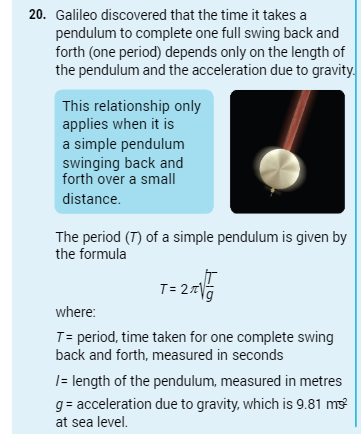
\includegraphics[width=.7\linewidth]{q20part1}\\
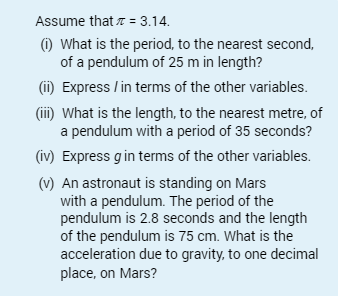
\includegraphics[width=.7\linewidth]{q20part2}

\newpage
\end{enumerate}

% Q16
\vspace*{7cm}
\item Identities / Unknown Coefficients \\[4pt]

\begin{enumerate}
\item{If $(x+t)^2$ = $x^2 + 6x + k$ for all values of x, find t and k.}\\
\noindent\fbox{\parbox{\linewidth}{
\begin{itemize}
\item[] Suggested Method:
\item Multiply out the brackets first.
\item Equate the left side to the right side.
\item Line up $x^2$ on left with $x^2$ on the right. Line up $x$ on left with $x$ on the right, and do the same for the constants.
\end{itemize}}}\\[3pt]
\newpage

\item{If $c(x-a)^2 +b = 3x^2 - 6x + 5$, find the values of a, b, c (where $a, b, c \in \!R $).}
\vspace{10cm}

\item{If $(x-3)$ and $(x-4)$ are factors of $x^3 + ax^2 + bx + c$, express b in terms of a and c in terms of b.}
\newpage

\item{If $x^2 -ax + b$ is a factor of $x^3 + cx + d$, prove (i) $b = a^2 + c$ and (ii) $d = a^3 + ac$}
\newpage

\item{If $x^2 -px + q$ is a factor of $x^3 + 3px^2 + 3qx + r$, show that $q = -2p^2$ and $r = -8p^3$}
\newpage
\vspace*{10cm}
\newpage

\item{$x^2 -ax + 2$ is a factor of $x^3 - x^2 + 5ax - b$}
\begin{enumerate}
\item{Express a in terms of b.}
\item{Find the value of a. Express your answer in surd form.}
\end{enumerate}
\newpage

\item{From 2011 Exam Paper: A cubic function is defined for x as $f(x) = x^3 + (1-k^2)x + k$, where k is a constant.}
\begin{enumerate}
\item{Show -k is a root.}
\item{Find in terms of k the other 2 roots.}
\end{enumerate}
\newpage
\end{enumerate}

% Q17
\item Problem Solving\\[4pt]
\noindent\fbox{\parbox{\linewidth}{
\begin{itemize}
\item[] Problem Solving Rules:
\item Read the question all the way through.
\item Identify an unknown value, and represent it with a letter (say x).
\item Most problems will consist of several unknown values, so let your letter (say x) represent the simplest of these.
\item Express all other unknown values in terms of this simplest value.
\item Convert the word equation into a mathematical equation.
\end{itemize}}}\\[3pt]

\begin{enumerate}
\item{Example p52}\\
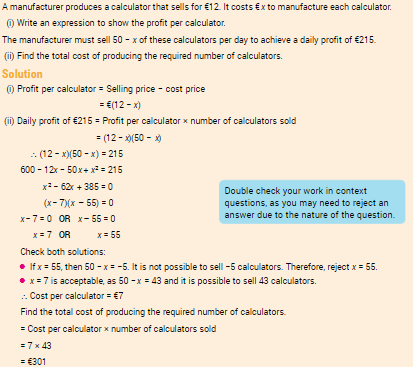
\includegraphics[keepaspectratio=true, scale=1.4]{examplep52}\\
\vspace{10cm}
\item{Q11 p55}\\
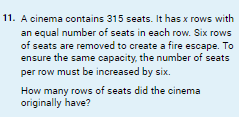
\includegraphics[width=.7\linewidth]{q11p55}\\
\newpage
\item{Q19 p56}\\
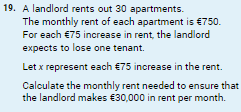
\includegraphics[width=.7\linewidth]{q19p56}\\
\vspace{10cm}
\item{Q22 p57}\\
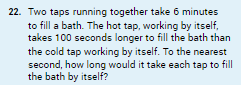
\includegraphics[width=.7\linewidth]{q22p57}\\
\newpage
\end{enumerate}


\vspace{10cm}
\end{enumerate}

 
\end{document}